\documentclass[11pt,compress,t,notes=noshow, aspectratio=169, xcolor=table]{beamer}

\usepackage{../../style/lmu-lecture}
% Defines macros and environments
% This file is included in slides and exercises

% Rarely used fontstyle for R packages, used only in 
% - forests/slides-forests-benchmark.tex
% - exercises/single-exercises/methods_l_1.Rnw
% - slides/cart/attic/slides_extra_trees.Rnw
\newcommand{\pkg}[1]{{\fontseries{b}\selectfont #1}}

% Spacing helpers, used often (mostly in exercises for \dlz)
\newcommand{\lz}{\vspace{0.5cm}} % vertical space (used often in slides)
\newcommand{\dlz}{\vspace{1cm}}  % double vertical space (used often in exercises, never in slides)
\newcommand{\oneliner}[1] % Oneliner for important statements, used e.g. in iml, algods
{\begin{block}{}\begin{center}\begin{Large}#1\end{Large}\end{center}\end{block}}

% Don't know if this is used or needed, remove?
% textcolor that works in mathmode
% https://tex.stackexchange.com/a/261480
% Used e.g. in forests/slides-forests-bagging.tex
% [...] \textcolor{blue}{\tfrac{1}{M}\sum^M_{m} [...]
% \makeatletter
% \renewcommand*{\@textcolor}[3]{%
%   \protect\leavevmode
%   \begingroup
%     \color#1{#2}#3%
%   \endgroup
% }
% \makeatother


\title{Interpretable Machine Learning}
% \author{LMU}
%\institute{\href{https://compstat-lmu.github.io/lecture_iml/}{compstat-lmu.github.io/lecture\_iml}}
\date{}

\begin{document}

\newcommand{\titlefigure}{figure/pdp_bike}
\newcommand{\learninggoals}{
\item Extrapolation and Interactions in PDPs
\item Centered ICE and PDP
}

\lecturechapter{PDP - Comments and Extensions}
\lecture{Interpretable Machine Learning}

\begin{frame}{Comments on Extrapolation}

% \begin{center}
% \includegraphics[width=0.8\textwidth]{figure_man/extrapolation01.png}
% \end{center}

Extrapolation can cause issues in regions with few observations or if features are correlated
 
\begin{columns}[T, totalwidth=\textwidth]
\begin{column}{0.5\textwidth}
\centering
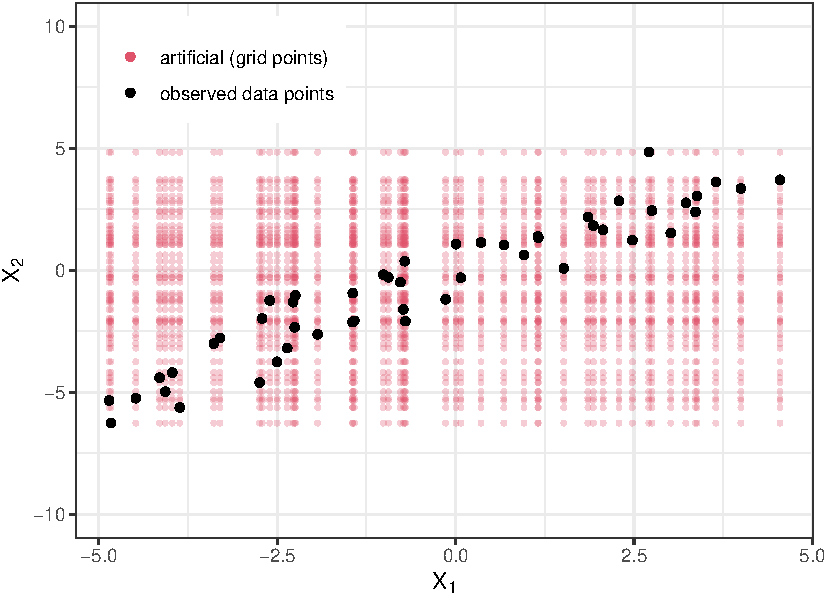
\includegraphics[width=0.8\textwidth]{figure/ale_scatter_grid}
\end{column}
\begin{column}{0.5\textwidth}
\centering
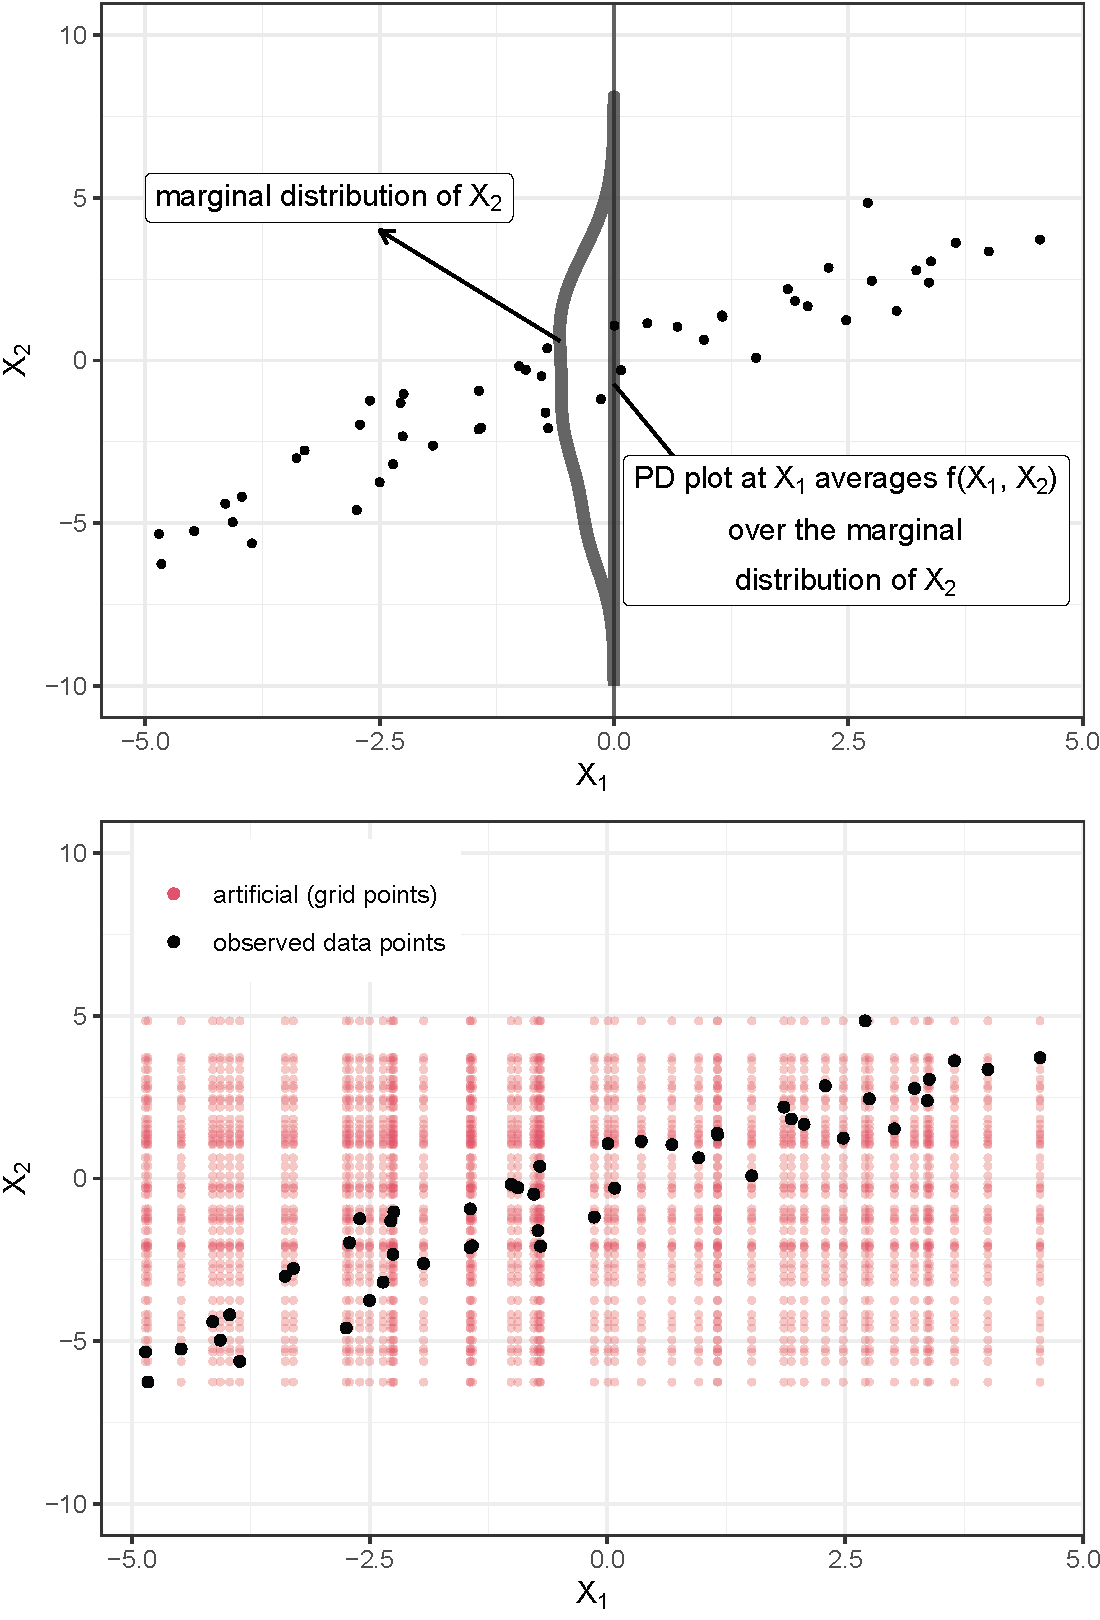
\includegraphics[width=0.8\textwidth]{figure/ale_pdplot}
\end{column}
\end{columns}

\begin{itemize}
\item \textbf{Example:} Features $x_1$ and $x_2$ are strongly correlated
\item \textbf{Black points:} Observed points of the original data
\item \textbf{\textcolor{red}{Red:}} Grid points to calculate the ICE and PD curves (many unrealistic values)\\ %combination of feature values
$\Rightarrow$ %Unrealistic combination of feature values are used, e.g., the
PD plot at $x_1=0$ averages predictions over the \textit{whole} marginal distribution of feature $x_2$\\
$\Rightarrow$ May be problematic if model behaves strange outside training distribution (e.g. model overfits)
%can bias ICE and PD curves Be careful with interpretations 
%\item For correlated features and in regions with few observations with care
%Extrapolation: interpret curves for highly correlated features and in feature regions with few observations with care
\end{itemize}

%
% \framebreak
%
%
% \begin{center}
% \includegraphics[width=0.8\textwidth]{figure_man/extrapolation02.png}
% \end{center}
%
% \begin{itemize}
% \item The features $x_1$ and $x_2$ are strongly correlated.
% \item \textcolor{red}{Red:} Observed points of the original data.
% \item \textcolor{green}{Green:} Grid points used to calculate the ICE and PD curves.
% \item Example: PD plot at $x_1=1.9$ averages predictions over the whole marginal distribution of feature $x_2$.
% \end{itemize}
\end{frame}




% \begin{frame}{Interactions}
%
% For PD plots, the averaging of ICE curves might \textbf{obfuscate} heterogeneous effects and interactions. \newline \(\Rightarrow\) Ideally plot ICE curves and PD plots together.
%
% \begin{center}\includegraphics[width=0.65\textwidth]{figure_man/pdp_xor.pdf} \end{center}
% %
% % \framebreak
% %
% % \begin{itemize}
% % \item
% %   For PD plots, the averaging of ICE curves might \textbf{obfuscate}
% %   heterogeneous effects and interactions. \newline \(\Rightarrow\)
% %   Ideally plot ICE curves and PD plots together.
% % \item
% %   \textbf{Extrapolation:} Interprete curves for highly correlated
% %   features and in feature regions with few observations with care.
% % \item
% %   Accumulated Local Effects (ALE) plots are a novel alternative to the PD plots developed by Apley (2020) that do not suffer from
% %   extrapolation in case of correlated features.
% % \end{itemize}
% %
% % \vspace{80pt}
% % \tiny{
% % Apley, D. W., \& Zhu, J. (2020). Visualizing the effects of predictor variables in black box supervised learning models. Journal of the Royal Statistical Society: Series B, 82(4), 1059-1086. \par}
% \end{frame}

\begin{frame}{Comments on Interactions}
\begin{itemize}
%\lz
%\item Accumulated Local Effects (ALE) plots are a novel alternative to PD plots developed by Apley (2016) that do not suffer from extrapolation in case of correlated features.

\item PD plots: averaging of ICE curves might \textbf{obfuscate} heterogeneous effects and interactions \\ 
\(\Rightarrow\) Ideally plot ICE curves and PD plots together to uncover this fact\\
\(\Rightarrow\) Different shapes of ICE curves suggest interaction (but do not tell with which  feature)

\begin{center}\includegraphics[width=0.5\textwidth]{figure/pdp_xor.pdf} \end{center}
\end{itemize}

%\footnote[frame]{Apley, Daniel W., and Jingyu Zhu (2020). Visualizing the Effects of Predictor Variables in Black Box Supervised Learning Models. Journal of the Royal Statistical Society: Series B (Statistical Methodology) 82.4: 1059-1086.}
\end{frame}

\begin{frame}{Comments on Interactions - 2D Partial Dependence}

\begin{center}
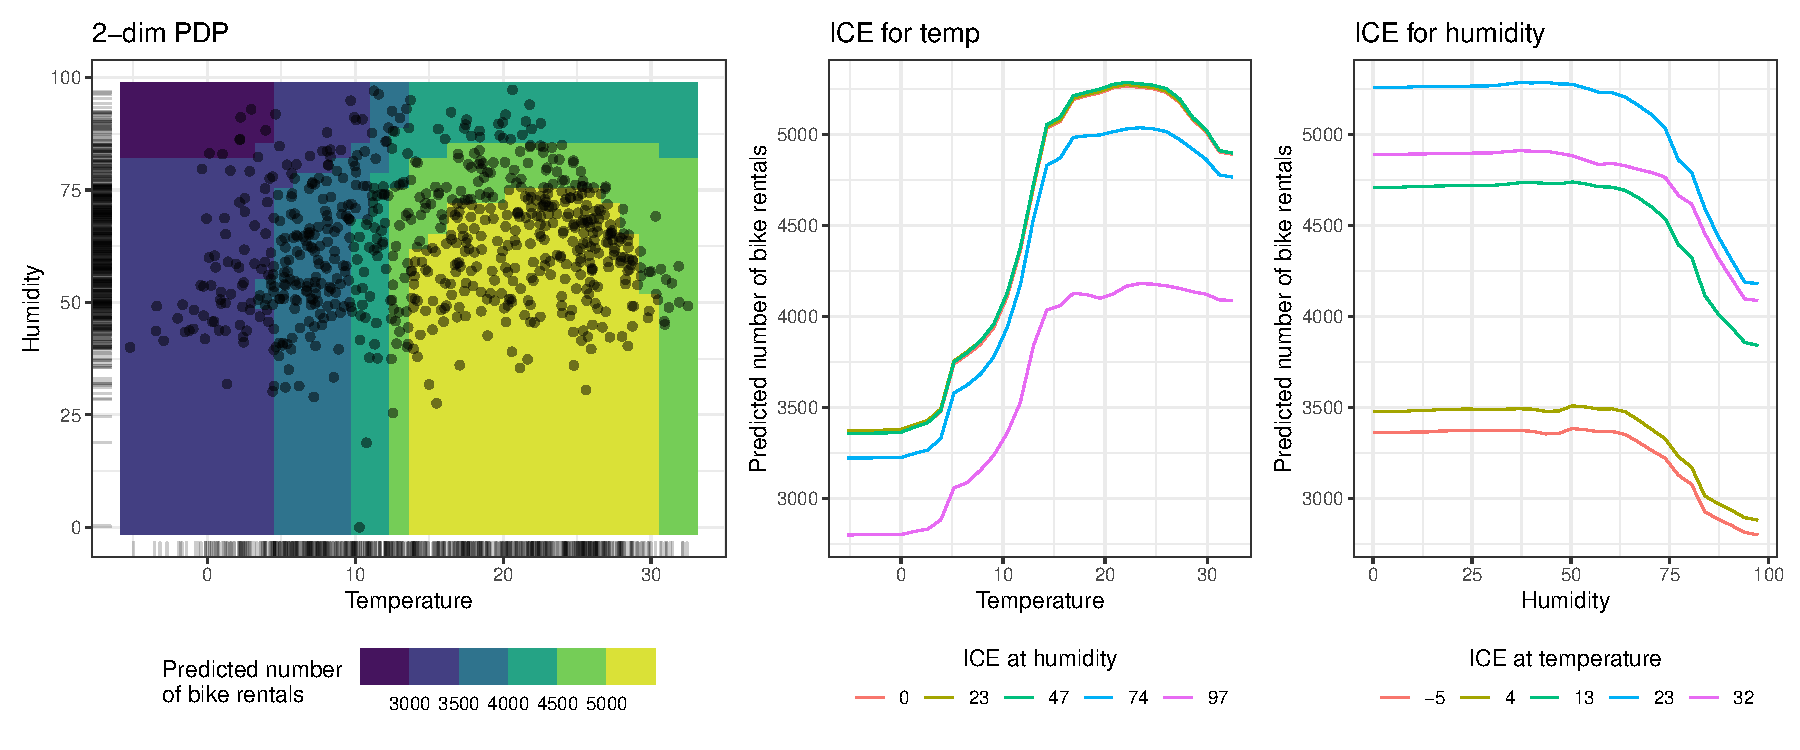
\includegraphics[width=0.9\textwidth]{figure/pdp2d_bike}
\end{center}

\begin{itemize}
 \item Humidity and temperature interact at high values (see shape difference)\\
 $\leadsto$ Shape of ICE curves at different horizontal and vertical slices varies (for high values)
 \item Low to medium humidity and high temperature $\Rightarrow$ many rented bikes
 %Many rented bikesThe number of bike rentals is especially high when humidity is below 75 percent and temperature is between 15 $^{\circ}$C and 27 $^{\circ}$C
\end{itemize}


% \framebreak
%
% add datapoints to previous figure and mention convex hull (see pdp package)

\end{frame}

\begin{frame}{Centered ICE Plot (c-ICE) \citebutton{Goldstein et al. (2015)}{https://doi.org/10.1080/10618600.2014.907095}}

\textbf{Issue:} Difficult to identify heterogenous ICE curves if curves have different intercepts (are stacked)
%When ICE curves start at different intercepts (are stacked), it is difficult to identify heterogenous predictions.

\textbf{Solution:} Center ICE curves at fixed reference value $x' \sim \P(\xv_S)$, often $x' = \min(\xv_S)$\\
$\Rightarrow$ Easier to identify heterogenous shapes with c-ICE curves
\vspace{-0.2cm}
\begin{columns}[c, totalwidth=\textwidth]
\begin{column}{0.45\textwidth}
%\centering
$$\begin{aligned}
\fh_{S, cICE}^{(i)}(\xv_S)
&= \fh(\xv_S, \xi_{-S}) - \fh(x', \xi_{-S}) \\
&= \fh_{S}^{(i)}(\xv_S) - \fh_{S}^{(i)}(x')
\end{aligned}$$

$\Rightarrow$ Visualize $\fh_{S, cICE}^{(i)}(\xv_S^*)$ vs. $\xv_S^*$

\lz
\pause
\textbf{Interpretation} \\
(yellow curve: analog to PDP the average of c-ICE curves): \\
On average, the number of bike rentals at $\sim 97$ \% humidity decreased by 1000 bikes compared to a humidity of 0 \%
\end{column}
\begin{column}{0.54\textwidth}
\begin{center}
%\vspace{-0.3cm}
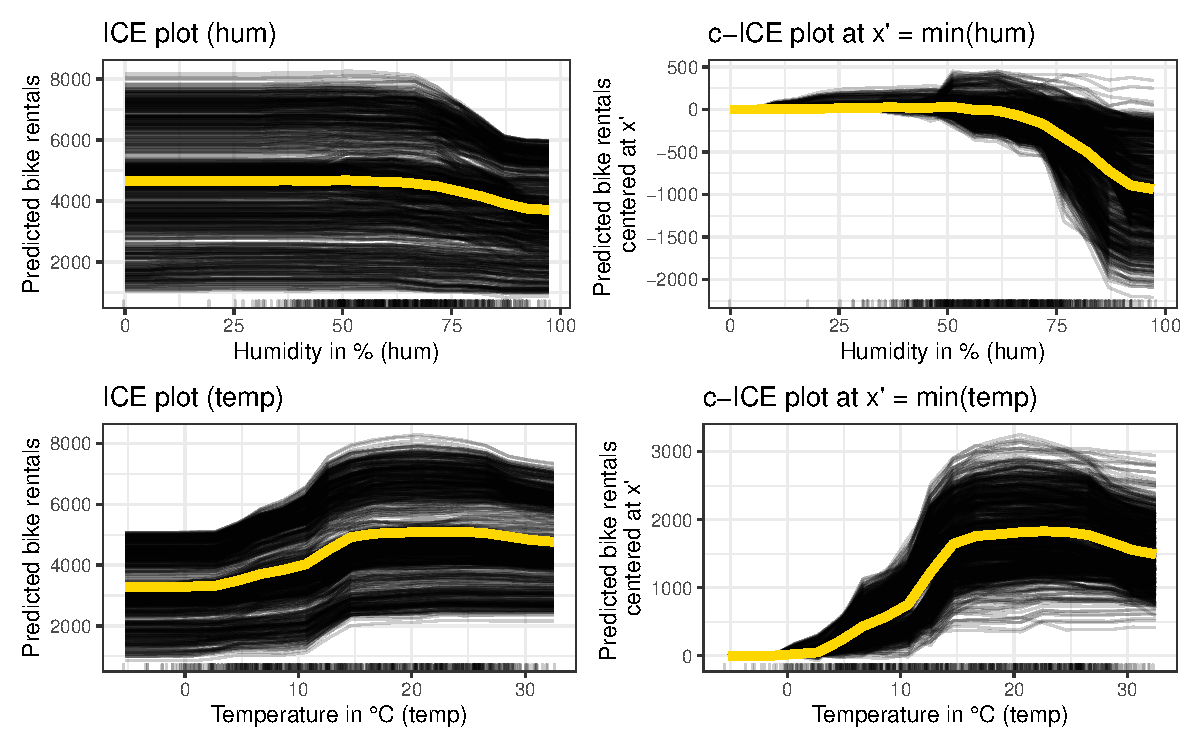
\includegraphics[width=\textwidth]{figure/cICE}
\end{center}
\end{column}
\end{columns}

%\vspace{-0.4cm}

\end{frame}


\begin{frame}{Centered ICE Plot (c-ICE)}

For categorical features, c-ICE plots can be interpreted as in LMs due to reference value

\begin{columns}[c, totalwidth=\textwidth]
\begin{column}{0.44\textwidth}

\begin{center}
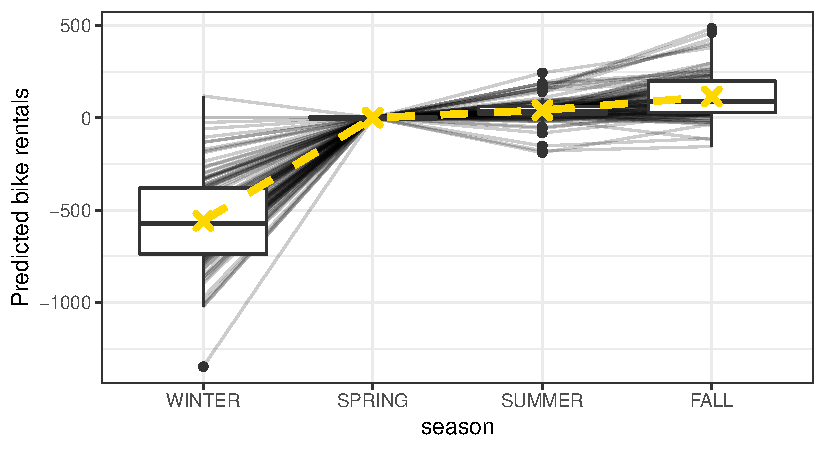
\includegraphics[width=\textwidth]{figure/cICEcat}
\end{center}

\end{column}
\begin{column}{0.55\textwidth}

\textbf{Interpretation}: \\
\begin{itemize}
%\item Centered ICE plots are useful for categorical features and can be interpreted as in LMs
\item The reference category is $x' =$ SPRING
\item Golden crosses: Average number of bike rentals if we jump from SPRING to any other season\\
$\Rightarrow$ Number of bike rentals drops by $\sim 560$ in \code{WINTER} and is slightly higher in \code{SUMMER} and \code{FALL} compared to \code{SPRING}
\end{itemize}

\end{column}
\end{columns}

\end{frame}


\endlecture
\end{document}
